% Version control information:
%$HeadURL: https://practicas-spss.googlecode.com/svn/trunk/introduccion_spss/introduccion_spss.tex $
%$LastChangedDate: 2010-09-27 16:37:11 +0200 (lun, 27 sep 2010) $
%$LastChangedRevision: 3 $
%$LastChangedBy: asalber $
%$Id: introduccion_spss.tex 3 2010-09-27 14:37:11Z asalber $

\chapter{Introducción a SPSS}

\section{Introducción}
La gran potencia de cálculo alcanzada por los ordenadores ha convertido a los mismos en poderosas herramientas al servicio de todas aquellas disciplinas que, como la estadística, requieren manejar un gran volumen de datos.
Actualmente, prácticamente nadie se plantea hacer un estudio estadístico serio sin la ayuda de un buen programa de análisis estadístico.

SPSS$^{\textsf{\textregistered}}$\renewcommand{\thefootnote}{\fnsymbol{footnote}}\footnote{Esta practica está basada en la versión 20.0 de SPSS$^{\textsf{\textregistered}}$ para Windows en español.} es uno de los programas de análisis estadísticos más utilizados, sobre todo en el ámbito de las ciencias biosanitarias.
\begin{center}
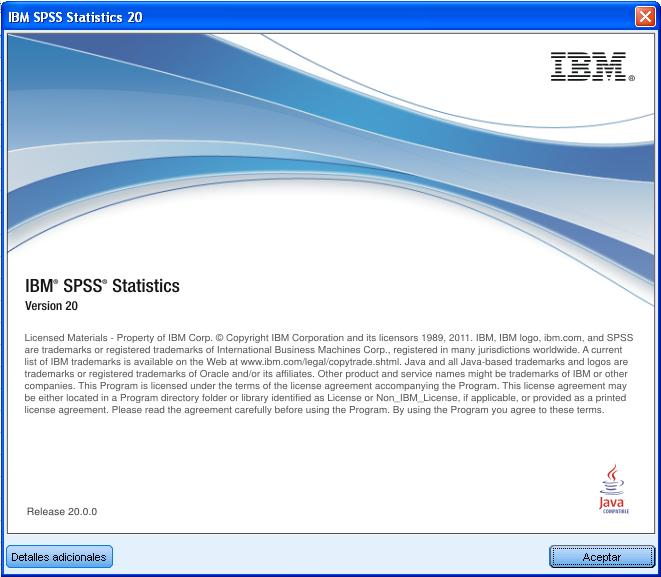
\includegraphics[scale=0.5]{introduccion_spss/img/portada}
\end{center}

El objetivo de esta práctica es introducir al alumno en la utilización de este programa, enseñándole a realizar las operaciones básicas más habituales. A lo largo de la práctica, los alumnos aprenderán a crear variables, introducir datos de las muestras, transformar variables, filtrar datos y fundir e importar archivos de datos.  


\section{Funciones básicas}
\subsection{Arranque}
Como cualquier otra aplicación de Windows, para arrancar el programa
hay que hacer click sobre la opción correspondiente del menú
\menu{Inicio\flecha Programas}, o bien sobre el icono de escritorio
\begin{center}
  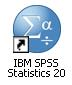
\includegraphics{introduccion_spss/img/icono}
\end{center}

Cuando el programa arranca, aparece la ventana del editor de datos (figura~\ref{g:vista_datos}).
\begin{figure}[h!]
\begin{center}
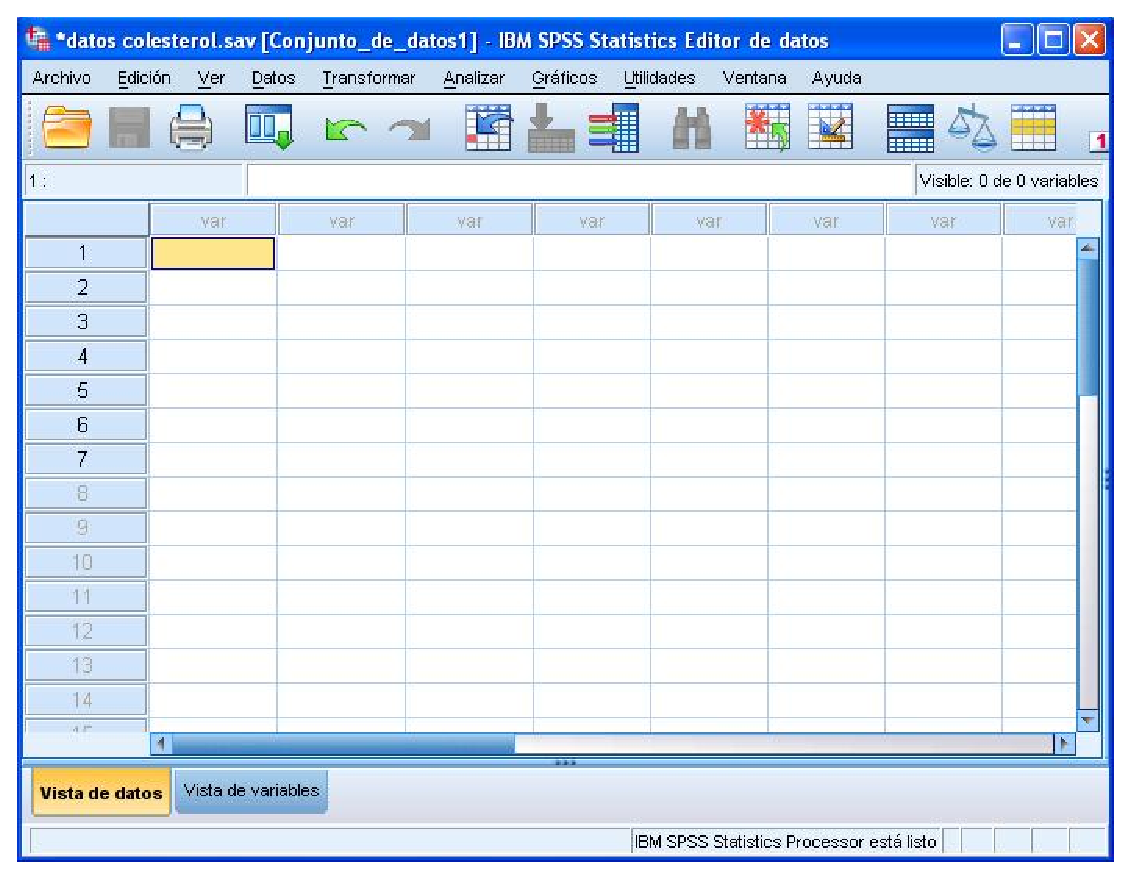
\includegraphics[scale=0.5]{introduccion_spss/img/vista_datos}
\caption{Ventana del editor de datos.}
\label{g:vista_datos}
\end{center}
\end{figure}
 
Como cualquier otra ventana de aplicación de Windows, la ventana del editor de datos tiene una barra de título, una barra de menús con las distintas funciones que puede hacer SPSS, entre ellas los análisis estadísticos de datos, una barra de botones que son atajos a las opciones más habituales de los menús, y una barra de estado en la parte inferior que nos indica lo que hace el programa en cada instante. Además, en la parte inferior aparecen dos pestañas que permiten pasar a la \opcion{Vista de datos} o a la \opcion{Vista de variables}.

\subsection{Introducción de datos}\label{s:introduccion_datos}
Para realizar cualquier análisis, la ventana del editor de datos debe contener la matriz de datos a analizar. Una vez que el usuario obtiene los datos muestrales, estos deben introducirse en esta ventana. Para ello, lo primero es definir las variables que se han considerado en el estudio. Cada variable se corresponderá con una columna de la matriz de datos. 

Para definir una variable debemos pasar a la \opcion{Vista de variables} haciendo click sobre la correspondiente pestaña (figura~\ref{g:vista_variables}). 

\begin{figure}[h!]
\begin{center}
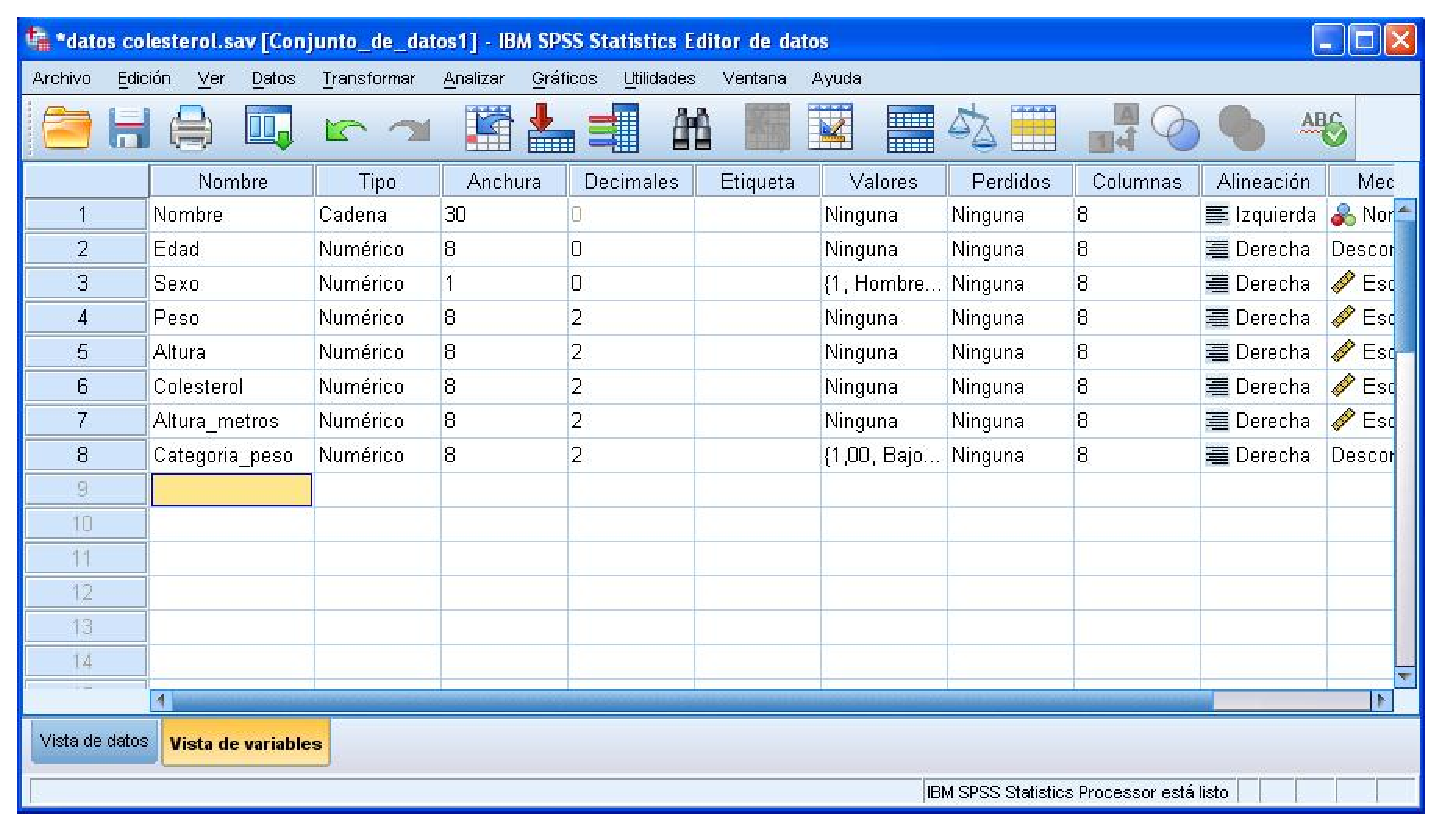
\includegraphics[scale=0.5]{introduccion_spss/img/vista_variables}
\caption{Vista de definición de variables.}
\label{g:vista_variables}
\end{center}
\end{figure}

En esta otra ventana, debemos definir cada variable en una fila, rellenando los siguientes campos:
\begin{description}
\item[Nombre] El nombre de la variable puede ser cualquier cadena de caracteres que comience por una letra y que no contenga espacios en blanco ni caracteres especiales como ?,¿,*, etc. Cada nombre de variable debe ser único y no se distingue entre mayúsculas y minúsculas. 
\item[Tipo] Los tipos más comunes son \texttt{Numérico} (formato numérico estándar), \texttt{Coma} (con comas de separación cada tres cifras y punto para la parte decimal), \texttt{Punto} (con puntos de separación cada tres cifras y coma para la parte decimal), \texttt{Notación Científica} (utiliza la E para la exponenciación), \texttt{Cadena} (para datos alfanuméricos) y \texttt{Fecha}.
\item[Anchura] Es el número máximo de caracteres que pueden tener los valores de la variable.
\item[Decimales] Para las variables numéricas es el número de cifras decimales que podrán escribirse.
\item[Etiqueta] Es una descripción de la variable. Si el nombre de la variable es suficientemente descriptivo se puede omitir. 
\item[Valores] Permite asignar etiquetas a los distintos valores que puede tomar la variable. No es obligatorio pero puede ser útil en algunos casos. 

Al hacer click sobre la casilla aparece un cuadro de diálogo para asignar etiquetas a valores. Para ello basta con escribir un valor en el cuadro de texto \opcion{Valor} y la correspondiente etiqueta en el cuadro de texto \opcion{Etiqueta}. Después hay que hacer click sobre el botón \boton{Añadir} y repetir los mismos pasos para todos los valores de la variable. Para finalizar hay que hacer click en el botón \boton{Aceptar}.
\item[Perdidos] Permite definir qué valores se utilizarán para representar los datos perdidos por el usuario. Es útil para distinguir datos que se han perdido por distintas causas. Por ejemplo, puede ser interesante distinguir el dato perdido correspondiente a un entrevistado que se niega a responder, del dato perdido debido a que la pregunta no le afectaba al entrevistado. Los valores de datos especificados como perdidos por el usuario se excluyen de la mayoría de los cálculos. 

Al hacer click sobre la casilla aparece un cuadro de diálogo donde deben indicarse los valores discretos que representarán valores perdidos (pueden introducirse hasta tres), o bien, el rango de valores que se representarán como valores perdidos. 

\item[Columnas] Permite especificar el ancho de la columna en la que se introducirán los datos correspondientes a la variable. 

\item[Alineación] Permite especificar la alineación de los datos correspondientes a la variable. Puede ser Izquierda, Derecha o Centrado. 

\item[Medida] Permite especificar el tipo de escala utilizada para medir la variable. Puede ser \opcion{Escala} cuando la variable es numérica y la escala es de intervalo, \opcion{Ordinal} cuando los valores de la variable representan categorías con un cierto orden o \opcion{Nominal} cuando los valores representan categorías sin orden.
\item[Rol] Permite especificar la función que una variable tiene en el análisis. Puede ser \opcion{entrada}, cuando se trata de una variable
independiente, \opcion{objetivo}, cuando es una variable dependiente, \opcion{ambos}, cuando la variable puede ser dependiente e
independiente, \opcion{ninguna} si la variable no tiene ninguna función asignada, \opcion{particion}, cuando la variable se utilizará para
dividir los datos en muestras separadas y \opcion{segmentar}, cuando se trata de una variable introducida para asegurar la compatibilidad en
SPSS.
\end{description}


Una vez definidas las variables se procede a introducir los datos de la muestra. Para ello hay que volver a la \opcion{Ventana de datos} haciendo click en la correspondiente pestaña. Ahora aparecerán en las cabeceras de columna los nombres de las variables definidas. Cada individuo de la muestra se corresponde con una fila de la matriz de datos. Para introducir el valor de una variable en un individuo determinado, nos situamos en la celda de la fila de dicho individuo y de la columna de la variable, bien haciendo click sobre la misma, o bien desplazándonos por la matriz de datos con las flechas de movimiento del cursor del teclado, y se teclea el valor seguido de la tecla \boton{Intro} (figura~\ref{g:matriz_datos}).

\begin{figure}[h!]
\begin{center}
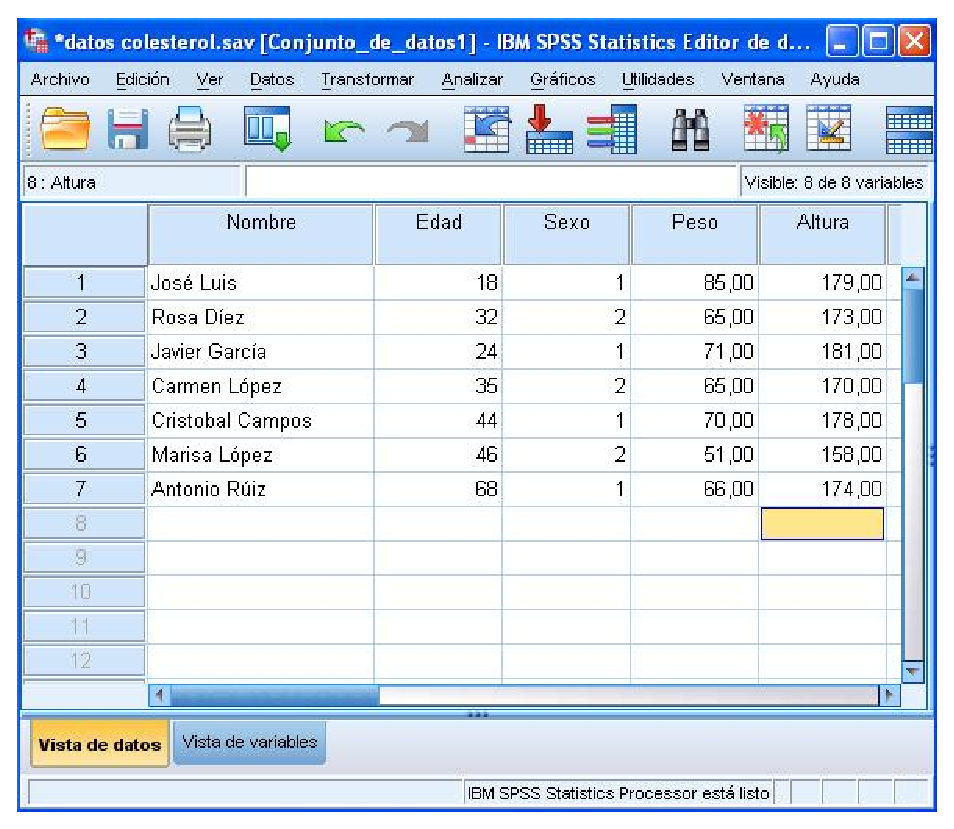
\includegraphics[scale=0.5]{introduccion_spss/img/matriz_datos}
\caption{Introducción de datos en la matriz de datos. Cada columna corresponde a una variable y cada fila a un individuo de la muestra.}
\label{g:matriz_datos}
\end{center}
\end{figure}

\subsection{Guardar datos}\label{s:guardar_datos}
Una vez introducidos los datos, conviene guardarlos en un fichero para no tener que volver a introducirlos en futuras sesiones. Para ello,
se selecciona el menú \menu{Archivo\flecha Guardar}. Si el fichero ya existe, se actualizará su información, y si no, aparecerá un cuadro de
diálogo en el que hay que introducir el nombre que queremos darle al fichero y la carpeta donde lo queremos ubicar. Los ficheros de datos de
SPSS tienen por defecto extensión \texttt{*.sav}. Cuando los datos estén guardados en un fichero, el nombre del fichero aparecerá en el
título de la ventana de datos (figura~\ref{g:matriz_datos}).

\subsection{Recuperar datos}
Si los datos con los que se pretende trabajar ya están guardados en un fichero, entonces tendremos que abrir dicho fichero. Para ello, se
selecciona el menú \menu{Archivo\flecha Abrir\flecha Datos} y se selecciona el fichero que se desea abrir. Automáticamente, los datos aparecerán
en la vista de datos.

\subsection{Modificación de datos}
En ocasiones es necesario modificar los datos de la matriz de datos para corregir errores, añadir nuevos datos o eliminarlos. Para corregir un valor basta con seleccionar la celda que contiene el valor y teclear el nuevo. Otras operaciones habituales son:
\begin{itemize}
\item Insertar una variable nueva entre otras ya existentes. En la vista de variables se selecciona la fila que contiene la variable por encima de la cual queremos insertar la nueva, y se selecciona el menú \menu{Edición\flecha Insertar variable}. 

\item Eliminar una variable. En la vista de variables se selecciona la fila que contiene la variable a eliminar y se pulsa la tecla \boton{Supr}.

\item Insertar un individuo entre otros ya existentes. En la vista de datos se selecciona la fila que contiene los datos del individuo por encima del cual queremos insertar el nuevo, y se selecciona el menú \menu{Edición\flecha Insertar caso}. 

\item Eliminar un individuo.  En la vista de datos se selecciona la fila que contiene los datos del individuo a eliminar y se se presiona la tecla \boton{Supr}. 
\end{itemize}

Cada vez que realicemos modificaciones en la matriz de datos, conviene volver a guardar los datos para que se actualice el fichero que los contiene.

\textbf{¡Importante!}: Cuando por equivocación realicemos una operación no deseada, podemos deshacerla mediante el menú \menu{Edición\flecha Deshacer}.

\subsection{Transformación y generación de datos}
En muchos análisis estadísticos se suelen transformar los datos de las variables originales en otros más convenientes para el análisis que se vaya a efectuar. Para generar una nueva variable mediante una transformación de otra ya existente o bien mediante funciones ya predefinidas se selecciona el menú \menu{Transformar\flecha Calcular Variable..}. Entonces aparece la ventana de transformación de variables tal y como se muestra en la figura~\ref{g:transformacion}.

\begin{figure}[h!]
\begin{center}
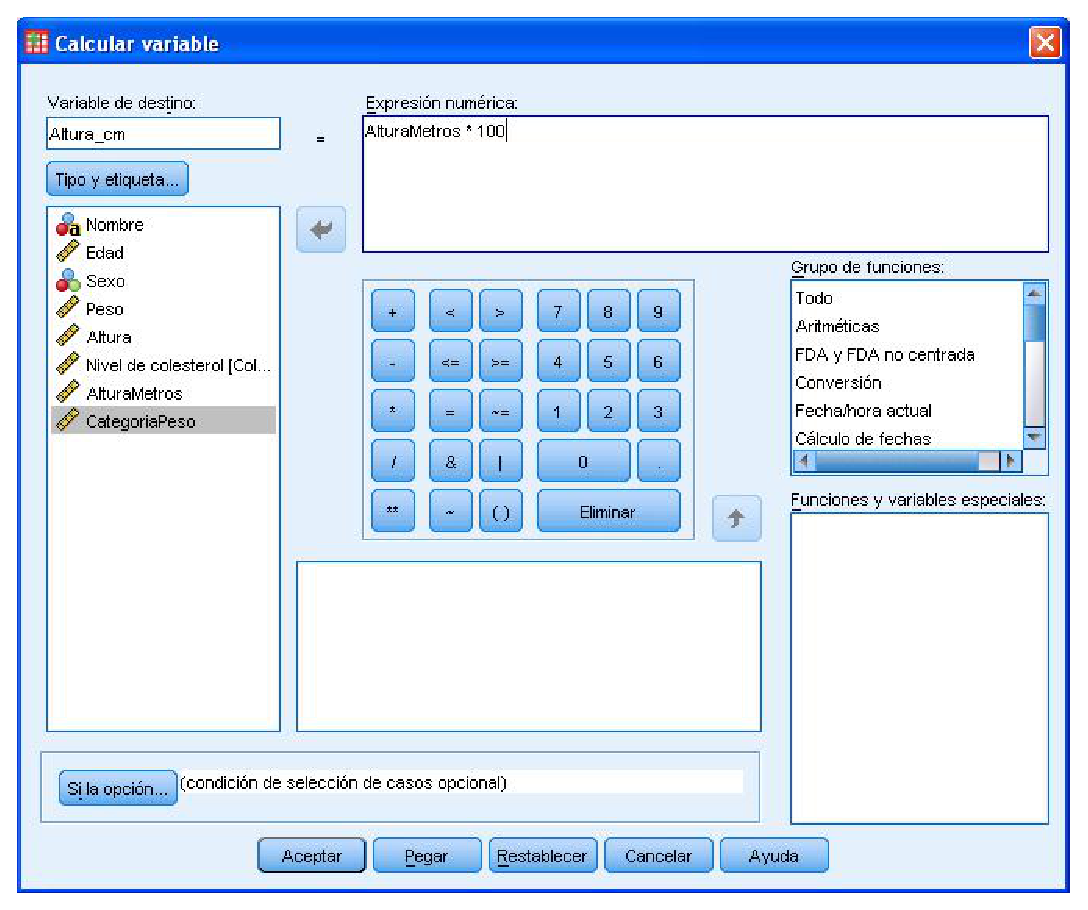
\includegraphics[scale=0.6]{introduccion_spss/img/transformacion}
\caption{Ventana de transformación de variables. A la izquierda aparecen las variables ya definidas, a la derecha las funciones predefinidas que pueden utilizarse, y en el centro los operadores aritméticos y relacionales más comunes.}
\label{g:transformacion}
\end{center}
\end{figure}

En esta ventana se debe introducir el nombre de la nueva variable en el cuadro \opcion{Variable de destino}, y la expresión cuyo resultado será el contenido de la nueva variable en el cuadro \opcion{Expresión numérica}. Para ello aparecen toda una serie de operadores y funciones para realizar la transformación, así como la lista de variables ya definidas que pueden utilizarse como argumentos de las distintas funciones de transformación.

Los operadores más habituales para construir expresiones son los aritméticos \texttt{+}, \texttt{-}, \texttt{*}, \texttt{/}, \texttt{**} (potenciación), los relacionales \texttt{=}, \texttt{<}, \texttt{>}, \verb"~=", \texttt{<=}, \texttt{>=} y los lógicos \texttt{\&} (Y), \texttt{|} (O) y \verb"~" (negación). Y algunas de las funciones más habituales son: \texttt{ABS} (valor absoluto), \texttt{SQRT} (raíz cuadrada), \texttt{EXP} (exponencial), \texttt{LN} (logaritmo neperiano), \texttt{SIN} (seno), \texttt{COS} (coseno), \texttt{TAN} (tangente), \texttt{SUM} (suma), \texttt{MEAN} (media aritmética), \texttt{SD} (desviación estándar), \texttt{RND} (redondeo al entero más cercano), \texttt{TRUNC} (parte entera de un número). 

Haciendo click en el botón \boton{Si la opción...} se pueden establecer condiciones de aplicación de la transformación. Para establecer una condición debemos activar la opción \opcion{Incluir si el caso satisface la condición} y  después introducir una condición lógica como por ejemplo \texttt{Sexo=1}. De este modo, la transformación sólo se aplicará a los individuos que cumplan dicha condición.

Una vez definida la expresión hay que hacer click sobre el botón \boton{Aceptar} y automáticamente aparecerá en la vista de datos una nueva columna con los datos transformados de la nueva variable. 

\subsection{Recodificación de datos}
Otra forma de transformar una variable es crear otra cuyos valores sean una recodificación de los de la primera, por ejemplo agrupando en intervalos. Esta recodificación podemos hacerla tanto en la misma variable como en variables diferentes. Para ello se selecciona el menú \menu{Transformar\flecha Recodificar en distintas variables}. Automáticamente aparece la ventana de recodificación de variables tal y como se ve en la figura~\ref{g:recodificacion}.

\begin{figure}[h!]
\begin{center}
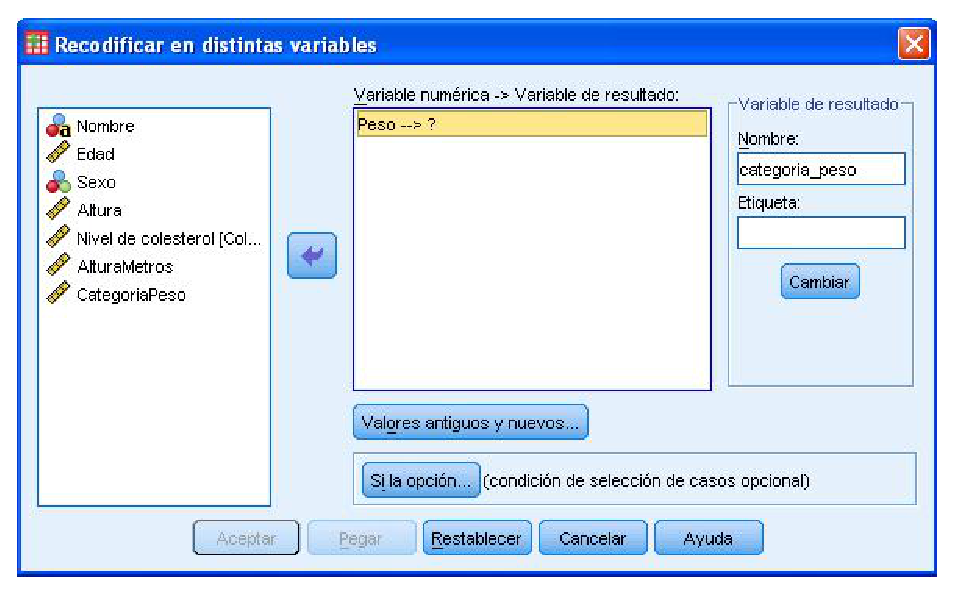
\includegraphics[scale=0.6]{introduccion_spss/img/recodificacion}
\caption{Ventana de recodificación de variables. A la izquierda aparecen las variables ya definidas, a la derecha deben especificarse las reglas de recodificación.}
\label{g:recodificacion}
\end{center}
\end{figure}

Para recodificar una variable en otra nueva, primero debemos seleccionar la variable que queremos recodificar y hacer click sobre el botón con una flecha que aparece al lado. Después hay que escribir el nombre de la nueva variable en el cuadro \opcion{Nombre} y hacer click sobre el botón \boton{Cambiar}. A continuación hay que establecer las reglas de recodificación. Para ello hay que hacer click en el botón \boton{Valores antiguos y nuevos} para que aparezca la ventana de definición de reglas (figura~\ref{g:definicion_intervalos}). Las reglas pueden establecer la conversión del valor de la variable original que introduzcamos en el cuadro \opcion{Valor antiguo} en el valor de la variable nueva que introduzcamos en el cuadro \opcion{Valor nuevo}, o bien la conversión de todo un intervalo de valores de la variable original en un valor de la variable nueva. Una vez definidos dichos valores hay que hacer click sobre el botón \boton{Continuar}, y después sobre \boton{Aceptar}.

\begin{figure}[h!]
\begin{center}
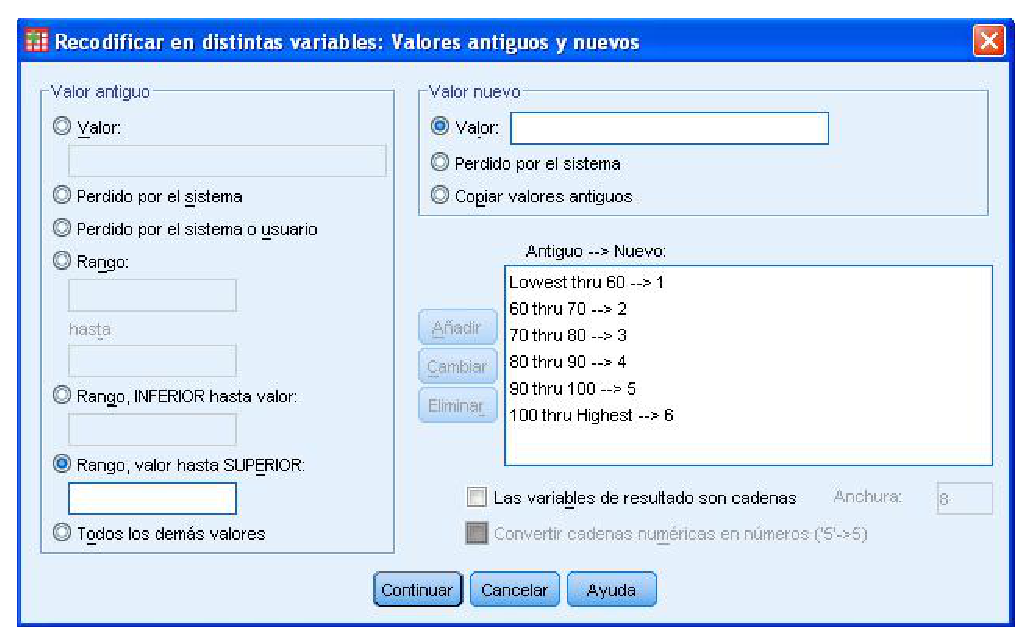
\includegraphics[scale=0.6]{introduccion_spss/img/definicion_intervalos}
\caption{Ventana de definición de reglas.}
\label{g:definicion_intervalos}
\end{center}
\end{figure}

\subsection{Impresión}
Para imprimir se utiliza el menú \menu{Archivo\flecha Imprimir}. Al instante aparece un cuadro de diálogo para la impresión donde debemos indicar si queremos imprimir todo o bien la selección que hayamos hecho. Tras esto se hace click sobre el botón \boton{Aceptar} y la información se envía a la impresora.

Antes de imprimir conviene hacer una previsualización de lo que se va a enviar a la impresora para estar seguros de que es eso lo que se
quiere. Para ello se utiliza el menú \menu{Archivo\flecha Presentación preliminar}. Entonces aparece un visor donde se ve la página, tal y como
se enviará a la impresora. Si todo parece correcto se puede hacer click sobre el botón \boton{Imprimir} y aparecerá el cuadro de diálogo de
impresión desde el que se puede enviar a la impresora definitivamente.

\subsection{Salir del programa}
Para terminar una sesión de trabajo se utiliza el menú \menu{Archivo\flecha Salir}, o bien se hace click sobre el aspa para cerrar la ventana del programa. Si quedan datos o resultados que no se han guardado, el programa nos preguntará antes de salir si deseamos guardarlos.

\subsection{Ayuda}
En esta práctica sólo hemos descrito las operaciones básicas en una sesión de trabajo. Pero quedan por describir todos los análisis estadísticos que pueden realizarse con los menús de la barra de menús. Aunque muchos de estos menús se explicarán en las siguientes prácticas, el programa dispone del menú de ayuda \menu{Ayuda} en el que podemos encontrar una descripción de todos estos menús y al que podemos recurrir cada vez que tengamos dudas.

\clearpage
\newpage

\section{Ejercicios resueltos}
\begin{enumerate}[leftmargin=*]
\item Introducir en la matriz de datos los datos de la siguiente muestra y guardarlos en un fichero con el nombre \texttt{datos\_colesterol.sav}.
\begin{center}
\begin{tabular}{|l|c|r|r|r|}
\hline
\multicolumn{1}{|c|}{Nombre} & \multicolumn{1}{c|}{Sexo} & \multicolumn{1}{c|}{Peso} & \multicolumn{1}{c|}{Altura} & \multicolumn{1}{c|}{Colesterol}\\
\hline
José Luis Martínez Izquierdo  & H &  85 & 179 & 182\\
Rosa Díaz Díaz & M & 65 & 173 & 232\\
Javier García Sánchez  & H & 71 & 181 & 191\\
Carmen López Pinzón & M &  65 & 170 & 200\\
Marisa López Collado & M &  51 & 158 & 148\\
Antonio Ruiz Cruz & H & 66 & 174 & 249\\
Antonio Fernández Ocaña & H &  62 & 172 & 276\\
Pilar Martín González & M &  60 & 166 & 213\\
Pedro Gálvez Tenorio & H &  90 & 194 & 241\\
Santiago Reillo Manzano & H &  75 & 185 & 280\\
Macarena Álvarez Luna & M &  55 & 162 & 262\\
José María de la Guía Sanz & H &  78 & 187 & 198\\
Miguel Angel Cuadrado Gutiérrez & H &  109  & 198 & 210\\
Carolina Rubio Moreno & M &  61 & 177 & 194\\
\hline
\end{tabular}
\end{center}


\begin{indicacion}
\begin{enumerate}
\item En la ventana de \opcion{Vista de variables}, crear las variables \variable{Nombre}, \variable{Sexo},  \variable{Peso}, \variable{Altura} y \variable{Colesterol} e introducir los datos anteriores, siguiendo las indicaciones del apartado~\ref{s:introduccion_datos}.

\item Una vez introducidos los datos, se guardan en un fichero de nombre \texttt{datos colesterol}
siguiendo lo indicado en el apartado~\ref{s:guardar_datos}.
\end{enumerate}
\end{indicacion}


\item Sobre la matriz de datos del ejercicio anterior realizar las siguientes operaciones:

\begin{enumerate}
\item Insertar detrás de la variable \variable{Nombre} una nueva variable \variable{Edad} con las edades
de todos los individuos de la muestra.
\begin{center}
\begin{tabular}{|l|r|}
\hline
\multicolumn{1}{|c|}{Nombre} & \multicolumn{1}{c|}{Edad} \\
\hline
José Luis Martínez Izquierdo & 18 \\
Rosa Díaz Díaz & 32 \\
Javier García Sánchez & 24 \\
Carmen López Pinzón & 35 \\
Marisa López Collado & 46 \\
Antonio Ruiz Cruz & 68 \\
Antonio Fernández Ocaña & 51 \\
Pilar Martín González & 22 \\
Pedro Gálvez Tenorio & 35 \\
Santiago Reillo Manzano & 46 \\
Macarena Álvarez Luna & 53 \\
José María de la Guía Sanz & 58 \\
Miguel Angel Cuadrado Gutiérrez & 27 \\
Carolina Rubio Moreno & 20 \\
\hline
\end{tabular}
\end{center}

\begin{indicacion}
\begin{enumerate}
\item En la \opcion{Vista de variables} seleccionar la fila correspondiente a la variable \variable{Sexo} haciendo click con el ratón sobre
la cabecera de la misma y a continuación seleccionar el menú \menu{Edición\flecha Insertar variable}, con lo que aparece una
nueva fila entre las variables \variable{Nombre} y \variable{Sexo}.
\item En la nueva fila definir la variable \variable{Edad} e introducir los datos anteriores.
\item En la \opcion{Vista de datos} rellenar los datos de la columna correspondiente a la \variable{Edad}.
\end{enumerate}
\end{indicacion}

\item Insertar entre los individuos 4º y 5º los datos correspondientes al siguiente individuo
\begin{quote}
Nombre: Cristóbal Campos Ruiz.\\
Edad: 44 años.\\
Sexo: Hombre.\\
Peso: 70 Kg.\\
Altura: 178 cm.\\
Colesterol: 220 mg/dl.
\end{quote}

\begin{indicacion}
\begin{enumerate}
\item Seleccionar la fila correspondiente al 5º individuo, haciendo click con el ratón sobre la cabecera de la misma y a continuación seleccionar el menú \menu{Edición\flecha Insertar caso}, con lo que aparece una nueva fila entre las correspondientes a los individuos 4º y 5º.
\item Introducir en la nueva fila los datos que se indican.
\end{enumerate}
\end{indicacion}


\item Cambiar el valor de la variable \variable{Peso} de Macarena Álvarez Luna por 58.
\begin{indicacion}
Hacer click con el ratón en la casilla cuyo contenido se desea modificar, escribir $58$ y pulsar \boton{Enter}.
\end{indicacion}

\item Transformar la variable \variable{Altura} para que aparezca expresada en metros.
\begin{indicacion}
\begin{enumerate}
\item Seleccionar el menú~\menu{Transformar\flecha Calcular variable}.
\item En la ventana de transformación de datos introducir el nombre \variable{Altura\_metros} en el cuadro \opcion{Variable de destino}.
\item Introducir la expresión \texttt{Altura/100} en el cuadro \opcion{Expresión numérica}.
\item Hacer click sobre el botón~\boton{Aceptar}. 
\end{enumerate}
\end{indicacion}

\item Recodificar la variable peso en las siguientes cuatro categorias, teniendo en cuenta el sexo:
\begin{center}
  \begin{tabular}{|l|c|c|}  
  \hline
    Categoria & Hombres & Mujeres \\
    \hline
    Bajo      &  $\leq 70$ & $\leq 60$ \\
    Medio     &  (70,85] & (60,70] \\
    Alto      &  (85,100] & (70,80] \\
    Muy Alto  &  $>100$ & $>80$ \\ 
    \hline
  \end{tabular}
\end{center}
\begin{indicacion}
\begin{enumerate}
\item Seleccionar el menú~\menu{Transformar\flecha Recodificar en distintas variables}.
\item En la ventana de recodificación de datos seleccionar la variable \variable{Peso} y hacer click sobre el botón con una flecha que aparece al lado. 
\item Escribir el nombre de la variable recodificada \texttt{Categoria\_Peso} en el cuadro \opcion{Nombre} de la \opcion{Variable de resultado} y hacer click sobre el botón \boton{Cambiar}. 
\item Hacer click en el botón \boton{Valores antiguos y nuevos} para abrir la ventana de definición de reglas de recodificación. 
\item Para definir las reglas de recodificación de los hombres,
\begin{enumerate}[i]
\item Seleccionar la opción \opcion{Rango INFERIOR hasta valor} del cuadro \opcion{Valor antiguo} e introducir 70 en el cuadro
correspondiente. Introducir 1 en el cuadro de la opción \opcion{Valor} del cuadro \opcion{Valor nuevo} y hacer click en el botón
\boton{Añadir}.
\item Seleccionar la opción \opcion{Rango} del cuadro \opcion{Valor antiguo} e introducir 70 en el cuadro correspondiente y 85 en el cuadro
\opcion{hasta}. Introducir 2 en el cuadro de la opción \opcion{Valor} del cuadro \opcion{Valor nuevo} y hacer click en el botón
\boton{Añadir}.
\item Seleccionar la opción \opcion{Rango} del cuadro \opcion{Valor antiguo} e introducir 85 en el cuadro correspondiente y 100 en el cuadro
\opcion{hasta}. Introducir 3 en el cuadro de la opción \opcion{Valor} del cuadro \opcion{Valor nuevo} y hacer click en el botón
\boton{Añadir}.
\item Seleccionar la opción \opcion{Rango valor hasta SUPERIOR} del cuadro \opcion{Valor antiguo} e introducir 100 en el cuadro
correspondiente. Introducir 4 en el cuadro de la opción \opcion{Valor} del cuadro \opcion{Valor nuevo} y hacer click en el botón
\boton{Añadir}.
\end{enumerate}
\item Hacer click en el botón \boton{Continuar} para cerrar la ventana. 
\item Hacer click en el botón \boton{Si la opción...} para abrir la ventana de definición de concidiones.
\item Seleccionar la opción \opcion{Incluir si el caso satisface la condición} e introducir la condición \texttt{Sexo=``H''} en el cuadro
correspondiente.
\item Hacer click en el botón \boton{Continuar} para cerrar la ventana.
\item Hacer click en el botón \boton{Aceptar}.
\item Repetir los mismos pasos para establecer las reglas de codificación de las mujeres.
\item En \menu{Vista de variables} hacer clik en \boton{Valores de Categoria\_Peso}, y en \opcion{Etiquetas de valor} ir asignando a los
valores $1$, $2$, $3$ y $4$ las etiquetas \texttt{Bajo}, \texttt{Medio}, \texttt{Alto} y \texttt{Muy alto} respectivamente, haciendo click
en el botón \boton{Añadir} después de cada asignación, y una vez terminado hacer click en el \boton{Aceptar}.
\end{enumerate}
\end{indicacion}

\item Volver a guardar los cambios en el fichero anterior y salir del programa.
\begin{indicacion}
\begin{enumerate}
\item Seleccionar el menú \menu{Archivo\flecha Guardar}.
\item Seleccionar el menú \menu{Archivo\flecha Salir}.
\end{enumerate}
\end{indicacion}

\end{enumerate}
\end{enumerate}

%\section{Caso práctico}
%Se ha diseñado un ensayo clínico aleatorizado, doble-ciego y
%controlado con placebo, para estudiar el efecto de dos
%alternativas terapéuticas en el control de la hipertensión
%arterial. Se han reclutado 100 pacientes hipertensos y estos han
%sido distribuidos aleatoriamente en tres grupos de tratamiento. A
%uno de los grupos (control) se le administró un placebo, a otro
%grupo se le administró un inhibidor de la enzima conversora de la
%angiotensina (IECA) y al otro un tratamiento combinado de un
%diurético y un Antagonista del Calcio. Las variables respuesta
%final fueron las presiones arteriales sistólica y diastólica.
%
%
%Los datos con las claves de aleatorización han sido introducidos
%en una base de datos que reside en la central de aleatorización,
%mientras que los datos clínicos han sido archivados en dos
%archivos distintos, uno para cada uno de los dos centros
%participantes en el estudio.
%
%Las variables almacenadas en estos archivos clínicos son las
%siguientes:
%
%\begin{itemize}
%\item CLAVE Clave de aleatorización
%\item NOMBRE  Iniciales del paciente
%\item F\_NACIM  Fecha de Nacimiento
%\item F\_INCLUS Fecha de inclusión
%\item SEXO  Sexo (0: Hombre 1: Mujer)
%\item ALTURA Altura en cm.
%\item PESO  Peso en Kg.
%\item PAD\_INI  Presión diastólica basal (inicial)
%\item PAD\_FIN  Presión diastólica final
%\item PAS\_INI Presión sistólica basal (inicial)
%\item PAS\_FIN  Presión sistólica final
%\end{itemize}
%
%El archivo de claves de aleatorización contiene sólo dos
%variables.
%
%\begin{itemize}
%    \item CLAVE Clave de aleatorización
%    \item FARMACO Fármaco administrado (0: Placebo, 1: IECA,  2:Ca Antagonista + diurético)
%\end{itemize}
%
%Se pide:
%
%\begin{enumerate}
%\item Leer los datos del centro con 10 pacientes, incluidos en el
%archivo \textsf{Hipertensos HA.xls}, este hospital trabaja con la
%hoja de cálculo Excel.
%
%\begin{indicacion}
%Desplegar el menú \menu{Archivo\flecha Abrir\flecha Datos}, e ir hasta el
%directorio que contiene el archivo \textsf{Hipertensos HA.xls},
%escogiendo como tipo de archivo el formato de Excel. Una vez tenemos
%delante el nombre del archivo, para abrirlo será suficiente con un
%doble clik, pero teniendo en cuenta que hay que activar la opción
%\opcion{Leer nombres de variables} si queremos que utilice la primera
%fila del archivo de Excel para dar nombre a las variables en el
%archivo de datos de SPSS.
%\end{indicacion}
%
%\item Añadir a estos, los datos de los pacientes 11 al 100,
%incluidos en el archivo \textsf{Hipertensos HB} y guardar los datos
%como \textsf{Hipertensos totales}.
%
%
%\begin{indicacion}
%\begin{enumerate}
%\item Teniendo en cuenta que lo que pretendemos es añadir nuevos casos
%a un archivo de datos ya abierto, el menú a utilizar es
%\menu{Datos\flecha Fundir archivos\flecha Añadir casos}. Después activamos la
%opción \opcion{Un archivo de datos de SPSS Statistics externo}, y con el botón
%\boton{Examinar} accedemos hasta la carpeta que contenga el archivo
%\textsf{Hipertensos HB}. Una vez seleccionado, utilizamos el botón
%\boton{Continuar}, y posteriormente el botón \boton{Aceptar} en el
%siguiente cuadro de diálogo que aparece.
%\item Una vez generado el archivo de datos, para guardarlo podemos
%utilizar el menú \menu{Archivo\flecha Guardar como}.
%\end{enumerate}
%\end{indicacion}
%
%\item Fusionar los datos clínicos con las claves de
%aleatorización. El fichero con las claves se denomina
%\textsf{Claves aleatorizacion}. Grabar el archivo resultante con
%el nombre \textsf{Hipertensos Datos Claves}
%
%\begin{indicacion}
%De forma similar al apartado anterior pero teniendo en cuenta que
%ahora lo que pretendemos es añadir variables. Para ello utilizamos el menú:
%\menu{Datos\flecha Fundir archivos\flecha Añadir variables}, para acceder
%después hasta el archivo \textsf{Claves aleatorizacion}, y
%posteriormente vamos aceptando en todos los cuadros de diálogo que
%aparecen. Una vez generado, guardamos el nuevo archivo de datos y
%claves: menú \menu{Archivo\flecha Guardar como}.
%\end{indicacion}
%
%\item Crear un archivo para cada uno de los grupos de tratamiento.
%Denominar a estos archivos \textsf{Hipertensos placebo},
%\textsf{Hipertensos IECA} e \textsf{Hipertensos Ca}
%respectivamente.
%
%\begin{indicacion}
%Se podría lograr el mismo resultado de múltiples maneras. Por
%ejemplo:
%\begin{enumerate}
%\item Segmentando el archivo mediante el menú \menu{Datos\flecha Dividir archivo...}, y \opcion{Organizar los resultados por grupos} basados en
%la variable \variable{farmaco}. Una vez dividido el archivo,
%podemos marcar los casos correspondientes a cada uno de los fármacos
%y hacer un cortar y pegar en un nuevo archivo específico para cada
%fármaco.
%\item También podemos generar los nuevos archivos utilizando el
%sistema de filtros de SPSS. Para ello el menú a utilizar es
%\menu{Datos\flecha Seleccionar Casos...}, con la opción \opcion{Si se
%satisface la condición}, botón \boton{Si la op...}, y entramos en un cuadro
%de diálogo en el que damos forma a la condición, que en primera
%instancia será \variable{farmaco=0}, para volver al cuadro de
%diálogo anterior y escoger la opción \opcion{Copiar casos seleccionados 
%a un nuevo conjunto de datos} y poner en \opcion{Nombre de 
%conjunto de datos:} \textsf{Hipertensos\_placebo}. Igualmente, 
%repetiríamos el proceso para los otros dos fármacos.
%\end{enumerate}
%\end{indicacion}
%
%\item Calcular, para cada paciente, la edad en años el día de la
%incorporación al estudio (redondeando al entero más próximo).
%Denominar la nueva variable \variable{edad} y etiquetarla
%correspondientemente.
%
%\begin{indicacion}
%Internamente SPSS trabaja con las variables en formato fecha
%almacenando el número de segundos transcurridos desde el comienzo
%del Calendario Gregoriano en el año 1582 hasta la fecha que
%introducimos. Por lo tanto, si restamos dos variables en formato
%fecha, no nos da el número de años transcurridos entre una y otra,
%sino el número de segundos. Por ello, la nueva variable obtenida
%como resultado de la resta hay que dividirla entre el número de
%segundos que tiene un año a razón de 3600 segundos la hora, 24 horas
%el día, y $365.25$ días el año, aproximadamente. Teniendo en cuenta
%lo anterior, el proceso a utilizar es: Menú
%\menu{Transformar\flecha Calcular variable}, y en \opcion{Variable de
%destino}, escribimos \variable{edad}. Como
%expresión numérica para su cálculo introducimos:
%
%\begin{center}
%\comando{(F\_INCLUS - F\_NACIM)/(365.25 * 24 * 3600)}
%\end{center}
%\end{indicacion}
%
%\item Recodificar dicha edad de forma que la nueva variable, de
%nombre \variable{grupoedad}, tome los siguientes valores y etiquetas
%de valor:
%
%\begin{center}
%
%\begin{tabular}{|l|l|l|}
%\hline
%\multicolumn{1}{|c|}{Edad en años} & \multicolumn{1}{c|}{Grupo edad} & \multicolumn{1}{c|}{Etiqueta} \\
%\hline
%\multicolumn{1}{|c|}{Edad $\leq 37$} & \multicolumn{1}{c|}{1} & \multicolumn{1}{c|}{Hasta 37 inclusive} \\
%\hline
%\multicolumn{1}{|c|}{$37<$ Edad $\leq 44$} & \multicolumn{1}{c|}{2} & \multicolumn{1}{c|}{De 37 a 44} \\
%\hline
%\multicolumn{1}{|c|}{$44<$ Edad $\leq 51$} & \multicolumn{1}{c|}{3} & \multicolumn{1}{c|}{De 44 a 51} \\
%\hline
%\multicolumn{1}{|c|}{Edad $>51$} & \multicolumn{1}{c|}{4} & \multicolumn{1}{c|}{Mayores de 51} \\
%\hline
%\end{tabular}
%
%\end{center}
%
%\begin{indicacion}
%Para recodificar una variable, se utiliza el proceso ya explicado en
%la práctica de Introducción a SPSS, con el menú
%\menu{Transformar\flecha Recodificar en distintas variables}, 
%escogiendo \variable{edad}
%como \opcion{Variable de entrada}, y dando el nombre 
%\variable{grupoedad} a la \opcion{Variable
%de resultado}, utilizando el botón \boton{Cambiar}, y posteriormente
%el botón \boton{Valores antiguos y nuevos} para delimitar las
%categorías de la nueva variable.
%\end{indicacion}
%
%
%
%
%\item Calcular, para cada paciente, el índice de masa corporal (se
%obtiene dividiendo el peso, expresado en kg, entre la altura,
%expresada en m, elevada al cuadrado) y almacenar el resultado en la
%variable \variable{masacorp}.
%
%\begin{indicacion}
%Con el menú \menu{Transformar\flecha Calcular variable}, escogiendo como
%variable de destino \variable{masacorp}, y como expresión numérica
%la indicada en el enunciado.
%\end{indicacion}
%
%\item Recodificar dicho índice de masa corporal, de forma que la
%nueva variable, de nombre \variable{obesidad}, tome los siguientes
%valores y etiquetas de valor según el sexo del paciente.
%
%\begin{center}
%\begin{tabular}{|l|l|l|l|}
%\hline
%\multicolumn{1}{|c|}{Sexo} & \multicolumn{1}{c|}{Masacorp} & \multicolumn{1}{c|}{Obesidad} & \multicolumn{1}{c|}{Etiqueta} \\
%\hline
%\multicolumn{1}{|c|}{} & \multicolumn{1}{c|}{$\leq 21$} & \multicolumn{1}{c|}{1} & \multicolumn{1}{c|}{Desnutrido} \\
%\cline{2-4}
%\multicolumn{1}{|c|}{} & \multicolumn{1}{c|}{$(21,\,26.94]$} & \multicolumn{1}{c|}{2} & \multicolumn{1}{c|}{Normal} \\
%\cline{2-4}
%\multicolumn{1}{|c|}{0} & \multicolumn{1}{c|}{$(26.94,\, 32.94]$} & \multicolumn{1}{c|}{3} & \multicolumn{1}{c|}{Sobrepeso} \\
%\cline{2-4}
%\multicolumn{1}{|c|}{} & \multicolumn{1}{c|}{$(32.94,\, 43.94]$} & \multicolumn{1}{c|}{4} & \multicolumn{1}{c|}{Obeso} \\
%\cline{2-4}
%\multicolumn{1}{|c|}{} & \multicolumn{1}{c|}{$>43.94$} & \multicolumn{1}{c|}{5} & \multicolumn{1}{c|}{Muy obeso} \\
%\hline
%\multicolumn{1}{|c|}{} & \multicolumn{1}{c|}{$\leq 19$} & \multicolumn{1}{c|}{1} & \multicolumn{1}{c|}{Desnutrido} \\
%\cline{2-4}
%\multicolumn{1}{|c|}{} & \multicolumn{1}{c|}{$(19,\, 24.94]$} & \multicolumn{1}{c|}{2} & \multicolumn{1}{c|}{Normal} \\
%\cline{2-4}
%\multicolumn{1}{|c|}{1} & \multicolumn{1}{c|}{$(24.94,\,29.94]$} & \multicolumn{1}{c|}{3} & \multicolumn{1}{c|}{Sobrepeso} \\
%\cline{2-4}
%\multicolumn{1}{|c|}{} & \multicolumn{1}{c|}{$(29.94,\,39.94]$} & \multicolumn{1}{c|}{4} & \multicolumn{1}{c|}{Obeso} \\
%\cline{2-4}
%\multicolumn{1}{|c|}{} & \multicolumn{1}{c|}{$>39,94$} & \multicolumn{1}{c|}{5} & \multicolumn{1}{c|}{Muy obeso} \\
%\hline
%\end{tabular}
%
%\begin{indicacion} 
%Se trata de un problema de recodificación, muy parecido al explicado en la indicación del punto 6, con la única novedad
%de que ahora hay que hacer una doble recodificación: por un lado para hombres y por el otro para mujeres. Para ello, después de escoger las
%variables de entrada y de resultado, haciendo uso del botón condicional \boton{Si la opción} podemos escoger únicamente los casos que
%cumplen la condición impuesta por la variable \variable{Sexo}; es decir, con la condición \variable{Sexo=0}, recodificamos en primera
%instancia el índice de masa corporal de los hombres, y con \variable{Sexo=1} recodificamos el de las mujeres.
%\end{indicacion}
%
%\end{center}
%
%\end{enumerate}
